\documentclass[a4paper, 10pt]{article}
\usepackage[utf8]{inputenc}
\usepackage[spanish]{babel}
\usepackage{graphicx}
\usepackage{geometry}
\usepackage{listings}
\usepackage{amsmath}
\usepackage{amsfonts}
\usepackage{amssymb}
\usepackage{caratula}

\newcommand{\Z}{\mathbb{Z}}
\def\code#1{\texttt{#1}}
\newcommand\tab[1][0.5cm]{\hspace*{#1}}

\geometry{a4paper, margin=0.7in}

\begin{document}
    %Caratula
    \pagenumbering{gobble}
    \newpage

    \begin{center}
        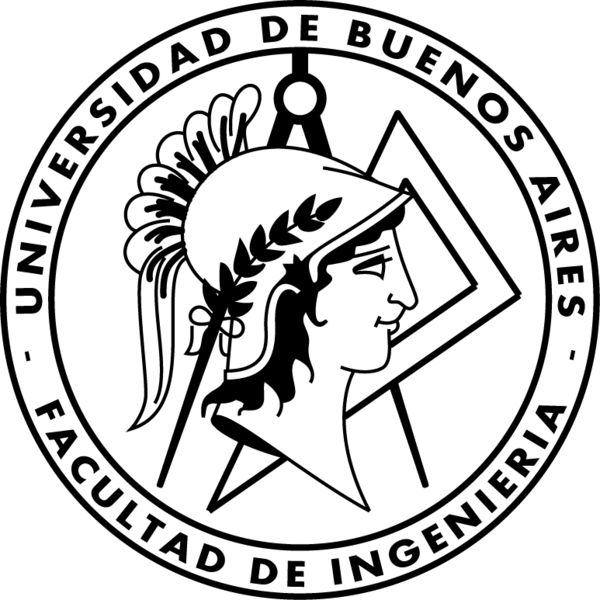
\includegraphics[width=5cm, height=5cm]{images/logo}
    \end{center}

    \materia{Teoría de Algoritmos I}
    \submateria{Primer Cuatrimestre 2017}
    \titulo{Trabajo Práctico 3}

    \integrante{Rodrigo De Rosa}{97799}{rodrigoderosa@outlook.com}
    \integrante{Marcos Schapira}{---}{schapiramarcos@gmail.com}
    \integrante{Facundo Guerrero}{97981}{facundoiguerrero@gmail.com}
    \maketitle
    %Fin caratula
    %Table of contents
    \newpage
    \pagenumbering{roman}
    \tableofcontents
    %Fin table of contents
    %Informe
    \newpage
    \pagenumbering{arabic}

    \section{Programación Dinámica}
        En esta sección se analiza una solución al problema de la predcción de acciones a través
        de la programación dinámica.
        \subsection{Algoritmo}
        \tab El algoritmo utilizado para resolver el problema planteado esta basado en el algoritmo de kadane.
             Este busca la maxima suma de elementos contiguos dentro de un arreglo.
             \subsubsection{Funcionamiento}
              \tab Este algoritmo funciona de la siguiente forma:
              \begin{itemize}
                \item Inicializa un \code{día de compra}, un \code{día de venta}, un \code{día de compra auxiliar}, todos
                  como el primer dia. Tambien se inicializa una \code{ganancia máxima} y una \code{ganancia temporal},
                  ambas como 0 ya que, hasta el momento, el dia de compra es igual al dia de venta.

                \item Luego itera sobre todos los días (valores diferentes de acciones) verificando si
                  en el día actual( dia i ) es más o menos favorable comprar acciones que en el día en el
                  que se pretendía hacerlo hasta el momento( dia k ), determinando el \code{día de compra auxiliar}.
                  Esto asegura la obtencion de la mayor ganancia hasta el dia i-1.

                \item A partir del día que determinó, calcula la \code{ganancia temporal} como la ganancia que se obtendría
                  si las acciones fueran compradas en el \code{día de compra} y vendidas el \code{día actual}.
                  Luego se verifica si la \code{ganancia temporal} es mayor a la \code{ganancia máxima}.

                \item En tal caso, determina el \code{día de venta} como el actual, el \code{día de compra}
                  como el que previamente era el \code{día de compra auxiliar} y la \code{ganancia máxima} como
                  la que era la \code{ganancia temporal}.

                \item Al finalizar la iteración, queda determinado el \code{día de compra} más conveniente, el
                  \code{día de venta} más conveniente y la \code{ganancia máxima} obtenible.

                \item Dado que el algoritmo propuesto recorre una sola vez el arreglo, funciona en $O(n)$.
              \end{itemize}

            \subsubsection{Ecuación de recurrencia}
                Para la ecuación de recurrencia se plantea lo siguiente: \\
                \begin{itemize}
                  \item Se tiene una variable \code{C_{i}} \code{= Día en el que se compran las acciones hasta el paso i, con i=1,...,n}.

                  \item Ademas, se tiene otra variable \code{V_{k}} \code{= Día en el que se venden las acciones hasta el paso k, con k=i,...,n}.

                  \item Observar que k esta relacionada con i, ya que el dia de venta debe ser mayor o igual al dia de compra. En el caso de ser igual, la ganancia seria 0.

                  \item Se puede obtener la \code{Ganancia Temporal} del paso \code{i,k}, como \code{GT_{i,k} = V_{k} - C_{i} }.

                  \item Entonces, la \code{Ganancia Máxima} es la máxima \code{ GT_{i,k} }.

                  \item Se puede definir la \code{Ganancia Máxima} para el paso \code{i,k} como:
                  \begin{center}
                    \tab\tab\tab\tab\tab\tab\tab\tab\code{GM_{i,k} } =
                    \begin{cases}
                      V_{k} - C_{i}  & \mbox{si } GT_{i,k} > GM_{i,k} \\
                      GT_{i,k-1} & \mbox{si } GT_{i,k} <= GM_{i,k}
                    \end{cases}
                  \end{center}
                \end{itemize}
    \newpage

    \section{Algoritmos Randomizados}
            En esta sección se analiza una solución al problema de hallar el corte global
        mínimo en un grafo no dirigido a través de un algoritmo randomizado.
        \subsection{Algoritmo}
                Para resolver este problema se utilizó el algoritmo de Karger descripto en
            la bibliografía proporcionada por la cátedra.
            \subsubsection{Funcionamiento}
                Sea el grafo $G = (E, V)$, el procedimiento del algoritmo es el siguiente:
                \begin{itemize}
                    \item Mientras $|V| > 2$:
                    \begin{itemize}
                        \item Se elige $e(u, v) \in E$ aleatoriamente.
                        \item Se crea un $w \in V$, el cual reemplaza tanto a $u$ como a $v$ en todas
                        las aristas en las que se encuentran. Es decir, $w$ puede tener más de una arista
                        que vaya a un mismo vértice $q \in V$.
                        \item Se elimina $e(u, v)$ de $E$.
                        \item Si existe alguna $e(v, v) \in E$ (arista de un vértice consigo mismo), se elimina.
                    \end{itemize}
                    \item Se devuelven las aristas que unen a esos dos vértices como el corte mínimo.
                \end{itemize}
            \subsubsection{Categoría de randomización}
                    Es un algoritmo \emph{Monte-Carlo} porque para algún orden de selección aleatoria
                de aristas, el corte obtenido \emph{no} es el mínimo. Es decir, es rápido siempre pero no siempre
                da resultados correctos. \\
                \tab La probabilidad de que este algoritmo devuelva un corte que sea mínimo es $p \geqslant \binom{n}{2}^{-1}$
                con $n = |V|$. Un dato adicional es que si el algoritmo se corre $T = \binom{n}{2}\ln{n}$ veces,
                la probabilidad de no encontrar un corte mínimo es $[1-p]^T \leqslant \dfrac{1}{n}$ en un tiempo
                $O(Tm) = O(n^2m\log{n})$ con $m = |E|$.
    \newpage

    \section{Algoritmos Aproximados}
        \tab En esta sección se analiza una solución al problema de la suma de subconjuntos
        a través de un algoritmo aproximado. Para resolver este problema se utilizó la
        estrategia polinómica descripta en la bibliografía proporcionada por la cátedra.
            \subsubsection{Funcionamiento}
                \tab El problema de la suma de subconjuntos (subset sum) consiste en, a partir de un conjunto S de enteros
                positivos y un target t también entero positivo, saber si existe algún subconjunto de S cuya suma sea
                exactamente t. Este problema es NP-Completo.
                \tab A partir de él se puede derivar a una aproximación completamente polinómica mediante el “recorte” o
                “trimming” de cada subconjunto que se va generando en el algoritmo exacto. Este mecanismo se sostiene de
                la idea de que si dos números pertenecen a S y tienen valores similares entonces no tiene mucho sentido
                mantener a ambos explícitamente (en referencia al algoritmo aproximado). Así es como mediante un parámetro
                de aproximación sigma tal que:
                                                            0 < sigma < 1
                \tab Se eliminan tantos elementos de S como sea posible ya que por cada elemento eliminado va a haber otro
                que pertenezca a S y lo represente. Así es como el algoritmo logra dado un conjunto S y un parámetro t
                devolver la mayor suma de elementos menor o igual a t. A la vez el algoritmo obtiene por parámetro a sigma,
                con lo cual la suma que devuelve está a un factor de (1 + sigma) del valor real.
            \subsubsection{Análisis del Algoritmo}
                \tab La tabla a continuación muestra resultados del algoritmo con sigmas variables. A la vez los elementos
                en cada instancia y el valor de t fueron generados aleatoriamente. Z es el valor devuelto por el algoritmo.

                \begin{table}[h!]
                    \centering
                    \caption{Resultados para N = 350}
                    \begin{tabular}{c|c|c|c}
                        T & Sigma & Zreal & Z real porcentual \\
                        \hline
                        2213 & 0,94 & 2211 & \%99,9 \\
                        \hline
                        2246 & 0,46 & 2245 & \%99,9 \\
                        \hline
                        2182 & 0,65 & 2182 & \%100 \\
                        \hline
                        2620 & 0,74 & 2618 & \%99,9 \\
                        \hline
                        173 & 0,62 & 172 & \%99,4 \\
                    \end{tabular}
                \end{table}

                \tab Como se puede apreciar, los porcentajes son extremadamente altos y caen dentro del factor esperado.
    \newpage

    \section{Ejecución de programas}
    \tab Para correr cada algoritmo, se debe ejecutar el archivo principal de cada uno.
    Esto se hace de la siguiente forma: \\
    \tab\tab En la carpeta \code{Programación Dinámica} abrir la consola y ejecutar \code{python main.py} \\
    \tab\tab En la carpeta \code{Algoritmos Randomizados} abrir la consola y ejecutra \code{python main.py} \\
    \tab\tab En la carpeta \code{Algoritmos Aproximados} abrir la consola y ejecutra \code{python main.py} \\

    %Fin informe
\end{document}
